% Options for packages loaded elsewhere
\PassOptionsToPackage{unicode}{hyperref}
\PassOptionsToPackage{hyphens}{url}
%
\documentclass[
]{article}
\usepackage[preprint]{neurips_2020}
\usepackage{booktabs}
\usepackage{fvextra}
\usepackage{amsmath,amssymb}
\usepackage{lmodern}
\usepackage{iftex}
\ifPDFTeX
  \usepackage[T1]{fontenc}
  \usepackage[utf8]{inputenc}
  \usepackage{textcomp} % provide euro and other symbols
\else % if luatex or xetex
  \usepackage{unicode-math}
  \defaultfontfeatures{Scale=MatchLowercase}
  \defaultfontfeatures[\rmfamily]{Ligatures=TeX,Scale=1}
\fi
% Use upquote if available, for straight quotes in verbatim environments
\IfFileExists{upquote.sty}{\usepackage{upquote}}{}
\IfFileExists{microtype.sty}{% use microtype if available
  \usepackage[]{microtype}
  \UseMicrotypeSet[protrusion]{basicmath} % disable protrusion for tt fonts
}{}
\makeatletter
\@ifundefined{KOMAClassName}{% if non-KOMA class
  \IfFileExists{parskip.sty}{%
    \usepackage{parskip}
  }{% else
    \setlength{\parindent}{0pt}
    \setlength{\parskip}{6pt plus 2pt minus 1pt}}
}{% if KOMA class
  \KOMAoptions{parskip=half}}
\makeatother
\usepackage{xcolor}
\IfFileExists{xurl.sty}{\usepackage{xurl}}{} % add URL line breaks if available
\IfFileExists{bookmark.sty}{\usepackage{bookmark}}{\usepackage{hyperref}}
\hypersetup{
  hidelinks,
  pdfcreator={LaTeX via pandoc}}
\urlstyle{same} % disable monospaced font for URLs
\usepackage{color}
\usepackage{fancyvrb}
\newcommand{\VerbBar}{|}
\newcommand{\VERB}{\Verb[commandchars=\\\{\}]}
\DefineVerbatimEnvironment{Highlighting}{Verbatim}{breaklines,fontsize=\scriptsize,commandchars=\\\{\}}
% Add ',fontsize=\small' for more characters per line
\newenvironment{Shaded}{}{}
\newcommand{\AlertTok}[1]{\textcolor[rgb]{1.00,0.00,0.00}{\textbf{#1}}}
\newcommand{\AnnotationTok}[1]{\textcolor[rgb]{0.38,0.63,0.69}{\textbf{\textit{#1}}}}
\newcommand{\AttributeTok}[1]{\textcolor[rgb]{0.49,0.56,0.16}{#1}}
\newcommand{\BaseNTok}[1]{\textcolor[rgb]{0.25,0.63,0.44}{#1}}
\newcommand{\BuiltInTok}[1]{#1}
\newcommand{\CharTok}[1]{\textcolor[rgb]{0.25,0.44,0.63}{#1}}
\newcommand{\CommentTok}[1]{\textcolor[rgb]{0.38,0.63,0.69}{\textit{#1}}}
\newcommand{\CommentVarTok}[1]{\textcolor[rgb]{0.38,0.63,0.69}{\textbf{\textit{#1}}}}
\newcommand{\ConstantTok}[1]{\textcolor[rgb]{0.53,0.00,0.00}{#1}}
\newcommand{\ControlFlowTok}[1]{\textcolor[rgb]{0.00,0.44,0.13}{\textbf{#1}}}
\newcommand{\DataTypeTok}[1]{\textcolor[rgb]{0.56,0.13,0.00}{#1}}
\newcommand{\DecValTok}[1]{\textcolor[rgb]{0.25,0.63,0.44}{#1}}
\newcommand{\DocumentationTok}[1]{\textcolor[rgb]{0.73,0.13,0.13}{\textit{#1}}}
\newcommand{\ErrorTok}[1]{\textcolor[rgb]{1.00,0.00,0.00}{\textbf{#1}}}
\newcommand{\ExtensionTok}[1]{#1}
\newcommand{\FloatTok}[1]{\textcolor[rgb]{0.25,0.63,0.44}{#1}}
\newcommand{\FunctionTok}[1]{\textcolor[rgb]{0.02,0.16,0.49}{#1}}
\newcommand{\ImportTok}[1]{#1}
\newcommand{\InformationTok}[1]{\textcolor[rgb]{0.38,0.63,0.69}{\textbf{\textit{#1}}}}
\newcommand{\KeywordTok}[1]{\textcolor[rgb]{0.00,0.44,0.13}{\textbf{#1}}}
\newcommand{\NormalTok}[1]{#1}
\newcommand{\OperatorTok}[1]{\textcolor[rgb]{0.40,0.40,0.40}{#1}}
\newcommand{\OtherTok}[1]{\textcolor[rgb]{0.00,0.44,0.13}{#1}}
\newcommand{\PreprocessorTok}[1]{\textcolor[rgb]{0.74,0.48,0.00}{#1}}
\newcommand{\RegionMarkerTok}[1]{#1}
\newcommand{\SpecialCharTok}[1]{\textcolor[rgb]{0.25,0.44,0.63}{#1}}
\newcommand{\SpecialStringTok}[1]{\textcolor[rgb]{0.73,0.40,0.53}{#1}}
\newcommand{\StringTok}[1]{\textcolor[rgb]{0.25,0.44,0.63}{#1}}
\newcommand{\VariableTok}[1]{\textcolor[rgb]{0.10,0.09,0.49}{#1}}
\newcommand{\VerbatimStringTok}[1]{\textcolor[rgb]{0.25,0.44,0.63}{#1}}
\newcommand{\WarningTok}[1]{\textcolor[rgb]{0.38,0.63,0.69}{\textbf{\textit{#1}}}}
\usepackage{graphicx}
\makeatletter
\def\maxwidth{\ifdim\Gin@nat@width>\linewidth\linewidth\else\Gin@nat@width\fi}
\def\maxheight{\ifdim\Gin@nat@height>\textheight\textheight\else\Gin@nat@height\fi}
\makeatother
% Scale images if necessary, so that they will not overflow the page
% margins by default, and it is still possible to overwrite the defaults
% using explicit options in \includegraphics[width, height, ...]{}
\setkeys{Gin}{width=\maxwidth,height=\maxheight,keepaspectratio}
% Set default figure placement to htbp
\makeatletter
\def\fps@figure{htbp}
\makeatother
\setlength{\emergencystretch}{3em} % prevent overfull lines
\providecommand{\tightlist}{%
  \setlength{\itemsep}{0pt}\setlength{\parskip}{0pt}}
\setcounter{secnumdepth}{-\maxdimen} % remove section numbering
\newlength{\cslhangindent}
\setlength{\cslhangindent}{1.5em}
\newlength{\csllabelwidth}
\setlength{\csllabelwidth}{3em}
\newlength{\cslentryspacingunit} % times entry-spacing
\setlength{\cslentryspacingunit}{\parskip}
\newenvironment{CSLReferences}[2] % #1 hanging-ident, #2 entry spacing
 {% don't indent paragraphs
  \setlength{\parindent}{0pt}
  % turn on hanging indent if param 1 is 1
  \ifodd #1
  \let\oldpar\par
  \def\par{\hangindent=\cslhangindent\oldpar}
  \fi
  % set entry spacing
  \setlength{\parskip}{#2\cslentryspacingunit}
 }%
 {}
\usepackage{calc}
\newcommand{\CSLBlock}[1]{#1\hfill\break}
\newcommand{\CSLLeftMargin}[1]{\parbox[t]{\csllabelwidth}{#1}}
\newcommand{\CSLRightInline}[1]{\parbox[t]{\linewidth - \csllabelwidth}{#1}\break}
\newcommand{\CSLIndent}[1]{\hspace{\cslhangindent}#1}
\ifLuaTeX
  \usepackage{selnolig}  % disable illegal ligatures
\fi

\title{Selective Coloring}
\author{Francisco Noya\\ \texttt{fnoya2@illinois.edu}\\
\And Mesay Taye\\ \texttt{mesayst2@illinois.edu} \\
}
\date{2022-05-06}

\begin{document}
\maketitle

In this project we implemented a tool to selectively and automatically
colorize the foreground of black and white photographs. The tool
consists of two main algorithms. First, a ViT-LSGAN network colorizes
the entire photograph. Second, a segmentation network segments the
foreground from the background. Lastly, colorized foreground is blended
with the original background to produce a distinctive image.

\hypertarget{approach-for-the-colorization-network}{%
\section{Approach for the Colorization
Network}\label{approach-for-the-colorization-network}}

For the colorization task we worked on the \textbf{Lab} colorspace. In
this space, the \textbf{L} channel contains the luminance or intensity
information, while the \textbf{ab} channels contain the color
information. Therefore, a neural network can be trained with the
\textbf{L} channel of regular color images as input. Its predictions
will be ``fake'' \textbf{ab} channels and its loss will be calculated
with the ``real'' \textbf{ab} channels.

After a short bibliographic review we found that although traditional
convolutional neural networks (CNNs) could produce results almost
indistinguishable from real color photos (Zhang et al., 2016),
\emph{Generative Adversarial Networks} or GANs (Goodfellow et al., 2014)
were the most proper approach for this kind of problem. This network
architecture contains two modules, a Generator and a Discriminator. Both
models are trained in paralell. The objective of the generator is to
produce outputs similar enough to the ground truth that can fool the
discriminator. The discriminator's objective is to properly tell the
ground truth from the discriminator output.

Since training this kind of networks requires large datasets and
computing time, we decided to use pretrained models that have been used
for other tasks such as object classification. We followed a tutorial
inspired by the \emph{pix2pix} paper (Isola et al., 2016) but instead of
training a naïve \emph{UNet} as the generator, it used a \emph{ResNet18}
network as the generator (\emph{Colorizing Black \& White Images with
u-Net and Conditional GAN --- a Tutorial}, n.d.). Similar to
\emph{pix2pix} we used a patch discriminator that splits the image in 26
square patches (depending on the image size) and produces a \emph{real}
or \emph{fake} prediction for each of them.

To try different approaches, we decided to use \emph{Transformers} in
place of the discriminator and the generator. \emph{Transformers} are a
special architecture of DNN that make extensive use of attention
mechanisms (Vaswani et al., 2017). Because of their ability to have
larger receptive fields compared to convolutional neural networks
(CNNs), they can track long-range dependencies within an image. These
attention based architectures have proven very effective in image
processing tasks and gave rise to Visual Transformers or \textbf{ViT}
(Dosovitskiy et al., 2020). We tried different architectures on our own
using ViTs either as generators or discriminators and measured a range
of metrics for each of them. Finally, we fine tune the loss function to
get the best results.

\hypertarget{dataset}{%
\subsection{Dataset}\label{dataset}}

For training and validation purposes we used a subset of the COCO
dataset of images (Lin et al., 2014) that is provided by the FastAI
framework (\emph{Fast.ai}, n.d.). We downloaded 10.000 images from this
dataset and randomly splited them into two sets: a training set with
8.000 images and a validation set with 2.000 images. Then we resized the
images so that they have manageable dimensions that allow feeding into
the different network architectures without requiring extremely high
computational resources or long times. Similar to (Isola et al., 2016)
data augmentation was achieved by flipping the images horizontally (this
is only done for the training set). We used 16 images on each batch that
goes through the network. Each image was converted to the \textbf{Lab}
colorspace and the channels adjusted float values between -1 and 1.

\hypertarget{model-improvement}{%
\subsection{Model improvement}\label{model-improvement}}

Our initial model was a variation of the original \emph{pix2pix} GAN in
which the generator was replaced by a pre-trained \emph{ResNet18}
\emph{UNet}. We then experimented with different visual transfomers as
discriminators and generators. Our final model, named
\textbf{ViT-LSGAN}, uses a ViT as the generator and least squared errors
instead of cross entropy as the loss function of the discriminator. The
results of all the intermediate models that we trained and tested can be
found in \textbf{``Supplemental Materials''}.

\hypertarget{loss-functions}{%
\subsection{Loss functions}\label{loss-functions}}

The loss function of the discriminator for each image is either the
binary cross entropy or the least squared errors between the predictions
and the ground truth. The ground truth is either \emph{real} if the real
\textbf{ab} channels were fed into the discriminator, or \emph{fake} if
the generated \textbf{ab} channels were used instead. The loss function
of the generator was the combination of the L1 error and the loss
function of the discriminator as if they were \emph{real} \textbf{ab}
channels. The intuition behind is that the generator ``wins'' every time
it fools the discriminator into assigning \emph{real} predictions to the
generated outputs.

\hypertarget{model-training-transfer-and-validation}{%
\subsection{Model Training, Transfer and
Validation}\label{model-training-transfer-and-validation}}

For implementing these models we worked in Python and Jupyter Notebooks
making extensive use of PyTorch and NumPy libraries. All the training
was done on a machine equipped with an NVIDIA K80 GPU, 4 vCPUs and 61 GB
of RAM (\emph{AWS EC2 p2.xlarge} instance). The transfer learning,
validation and metrics calculation were done in an Intel Core i5 8th
generation CPU with 8 GB of RAM. For validation we used the 2000 images
from the \textbf{COCO} dataset that were not used for training, and a
set of 70 photographs that were taken by the authors. To assess the
different networks architectures we selected the following set of
metrics for regression models:

\begin{itemize}
\tightlist
\item
  Correlation coeficient \emph{R} squared
\item
  Explained variance
\item
  Mean absolute error
\item
  Median absolute error
\item
  Mean squared error
\end{itemize}

We calculated all these metrics for each one of the \textbf{ab}
channels.

\hypertarget{approach-for-image-segmentation}{%
\section{Approach for image
segmentation}\label{approach-for-image-segmentation}}

For foreground extraction, we first considered traditional approaches
including grabcut, graphcut, and combinations thereof. However, when
taking into account the fact that a) the categories of foreground
objects (portraits) are well identified beforehand b) the accuracy of
region segmentation should be optimized even in fairly complex
backgrounds c) fully automated foreground segmentation, when possible,
is likely to be preferable, we decided that deep neural network based
segmentation methods were better candidates for this job.

After conducting literature review and experimentation with various
architectures, we chose the Deeplabv3 network (Chen et al., 2017).

\hypertarget{what-is-deeplabv3}{%
\subsection{What is Deeplabv3?}\label{what-is-deeplabv3}}

Deeplabv3 is a deep convolutional network, ResNet-101-based in our case,
which introduces a number of important concepts that distinguish it from
conventional ConvNets and make it more suitable for semantic
segmentation. First, Deeplabv3 employs atrous/dilated convolution for
filters. This allows it to leverage wider field of view without
increasing the number of parameters, and thus the amount of computation,
involved. Second, Deeplabv3 uses atrous spatial pyramid pooling (ASPP)
to capture objects at multiple scales. It does so by stacking together
filters of various sampling rates. Figure \ref{fig:atrous} shows filters with
different sampling rates (Chen et al., 2018).

\begin{figure}
\centering
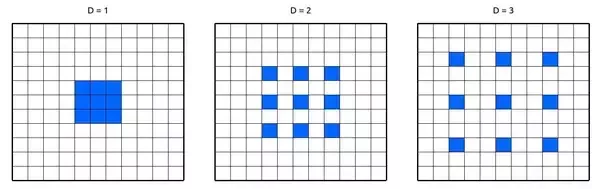
\includegraphics{report_images/atrous-conv.png}
\caption{Atrous/dilated convolutions (from https://www.mdpi.com).}
\label{fig:atrous}
\end{figure}

When sampling rate (represented by D in the image) is greater than one,
the convolution is considered atrous/dilated.

\begin{figure}
\centering
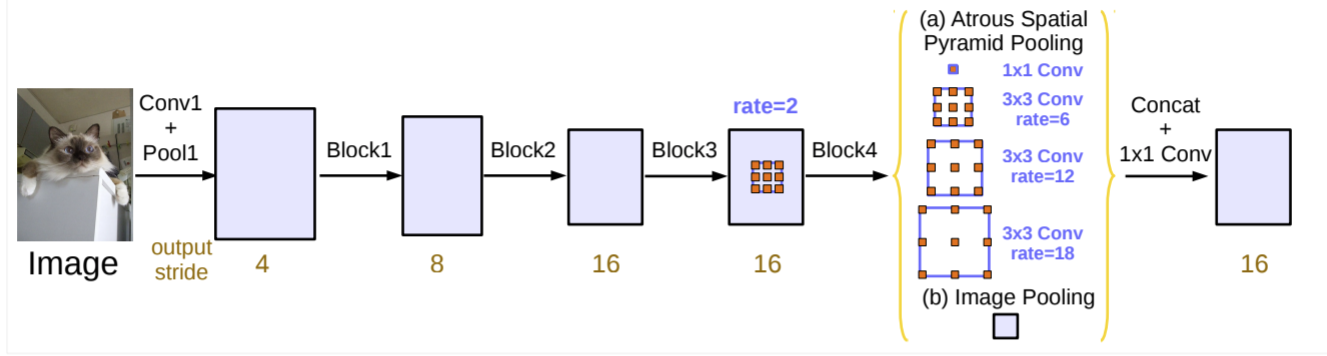
\includegraphics{report_images/deeplabv3.png}
\caption{DeeplabV3 architecture (Chen et al., 2017).}
\label{fig:deeplabv3}
\end{figure}

The loss function used by the Deeplabv3 is the sum of cross-entropy
terms for each spatial position for the output map. Using
ImageNet-pretrained ResNet-101 as a backend, and augmenting it with
Atrous convolutions followed by ASPP, DeeplabV3 achieves state-of-art
segmentation results on PASCAL-Context, PASCAL-Person-Part, and
Cityscapes (Chen et al., 2018) (Figure \ref{fig:deeplabv3}). It also performs similarly well on
random images as evidenced by the experiments in this project.

Our choice to use Deeplabv3 has been primarily informed by the
performance on PASCAL VOC 2012 in terms of pixel intersection-over-union
(mIoU). Table \ref{table:miou} shows the relative performance of Deeplabv3
vis-a-vis other comparable models (Chen et al., 2018).

\begin{table}\centering\caption[Pixel intersection-over-union metrics (mIoU) of segmentation models on PASCAL VOC 2012 dataset.]{mIoU of segmentation models}\label{table:miou}\begin{tabular}{ll}
\toprule{}                 Segmentation Method &              mIoU \\
\midrule    Adelaide VeryDeep FCN VOC  & 79.1 \\
LRR 4x ResNet-CRF          & 79.3 \\
DeepLabv2-CRF              & 79.7 \\
CentraleSupelec Deep G-CRF & 80.2 \\
HikSeg COCO                & 81.4 \\
SegModel                   & 81.8 \\
Deep Layer Cascade (LC)    & 82.7 \\
TuSimple                   & 83.1 \\
Large Kernel Matters       & 83.6 \\
Multipath-RefineNet        & 84.2 \\
ResNet-38 MS COCO          & 84.9 \\
PSPNet                     & 85.4 \\
IDW-CNN                    & 86.3 \\
CASIA IVA SDN              & 86.6 \\
DIS                        & 86.8 \\
DeepLabv3                  & 85.7 \\\bottomrule\end{tabular}\end{table}

\hypertarget{binary-mask-generation-and-image-blending}{%
\subsection{Binary mask generation and image
blending}\label{binary-mask-generation-and-image-blending}}

To produce the final blended image, we used the following procedure:

\begin{enumerate}
\def\labelenumi{\arabic{enumi}.}
\tightlist
\item
  Generate a segment map using Deeplabv3
\item
  Convert the segment map into binary mask
\item
  Create reverse mask from the binary mask
\item
  Multiply the colorized input image by the binary mask to get the
  colorized foreground
\item
  Multiply the grayscale image by the reverse mask to get the grayscale
  background
\item
  Create a new image by adding the foreground and the background images
\end{enumerate}

See details of the code in the \textbf{Supplementary Materials} section.

\hypertarget{results}{%
\section{Results}\label{results}}

\hypertarget{validation-of-colorization-models}{%
\subsection{Validation of colorization
models}\label{validation-of-colorization-models}}

\begin{figure}
\centering
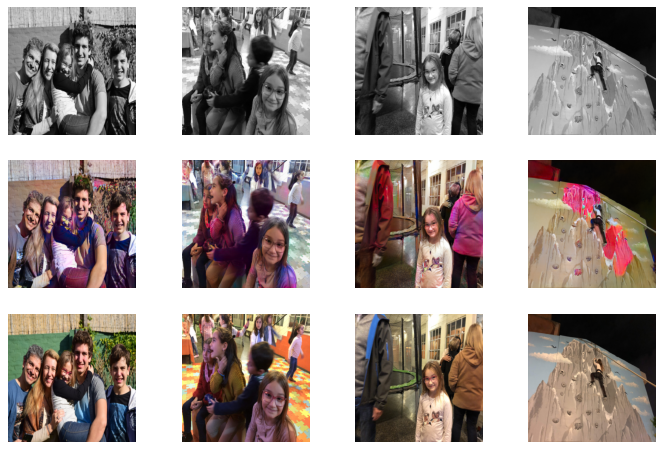
\includegraphics{results/ResNet18.png}
\caption{Samples of results from using a ResNet18 network as the
generator. Top row: inputs, Middle row: predictions, Bottom row: ground
truth.}
\label{fig:resnet18}
\end{figure}

\begin{table}\centering\caption[Metrics of ResNet18 generator on validation dataset]{ResNet18 metrics on validation dataset}\label{table:resnet18-metrics}\begin{tabular}{llll}\toprule{}                 Metric &              a-channel &             b-channel \\\midrule                R-square &     0.9762 &    0.7944 \\     Explained variance &     0.9763 &    0.8047 \\    Mean absolute error &   0.0221 &   0.0813 \\  Median absolute error &   0.0115 &  0.0533 \\     Mean squared error &  0.0016 &  0.0144 \\            Sample size &                   2000 &                  2000 \\\bottomrule\end{tabular}\end{table}

The results of the initial colorization model with a ResNet18 generator
were acceptable (Figure \ref{fig:resnet18}). However, many times the produced images did not look
natural because of an excessive use of colors that resulted in blotches
in the pictures. In agreement with the visual inspection, the resulting
metrics on the validation dataset (Table \ref{table:resnet18-metrics}) showed that the network did a pretty
good job at predicting the \textbf{a}-channel with over 97\% of the
variance of the channel predicted by the model with a very low mean
squared error. However, the prediction on the \textbf{b}-channel was not
as good with the model predicting only 80\% of its variance.

As explained before, to improve this results we tried variations of the
GAN using \emph{Transformers}. We experimented with the architectures summarized in Table \ref{table:architectures}. The description of each one and their results can be
found in the \textbf{Supplementary Materials} section.

\begin{table}\centering\caption[GAN architectures trained and validated in this work.]{GAN architectures trained and validated in this work.}\label{table:architectures}\begin{tabular}{ll}
\toprule{}                 GAN architecture & Summary of results\\
\midrule    
ResNet18 UNet as generator & Patches of colors, modest b-channel predictions.\\
ViT as discriminator       & Gray images.    \\
ViT as generator           & Gray images.    \\
ViT-LSGAN                  & Good natural colorization, best metrics for ab-channels.  \\
\bottomrule\end{tabular}\end{table}

In particular, the results from ViT-LSGAN model were very encouraging.  We got good results on our own photographies (Figure \ref{fig:ViT-LSGAN-results}) as well as in the COCO dataset ones (Figure \ref{fig:ViT-LSGAN-results-coco}). By using visual
transformers we got an improvement over the initial UNet based model on
every metric in particular in the \textbf{b}-channel which was the most
difficult to predict (Table \ref{table:ViT-LSGAN-metrics}). For example, this model was able to explain 98\%
of the variance of the \textbf{a}-channel and 86\% of the variance of
the \textbf{b}-channel, against 97\% and 80\%, respectively, when using
the UNet model.

\begin{figure}
\centering
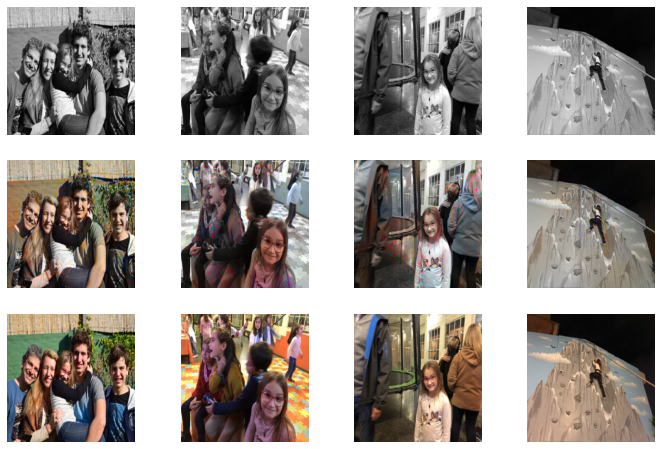
\includegraphics{results/FINAL_ViT_generator.png}
\caption{Samples of results of the ViT-LSGAN model. Top row: inputs,
Middle row: predictions, Bottom row: ground truth.}
\label{fig:ViT-LSGAN-results}
\end{figure}

\begin{figure}
\centering
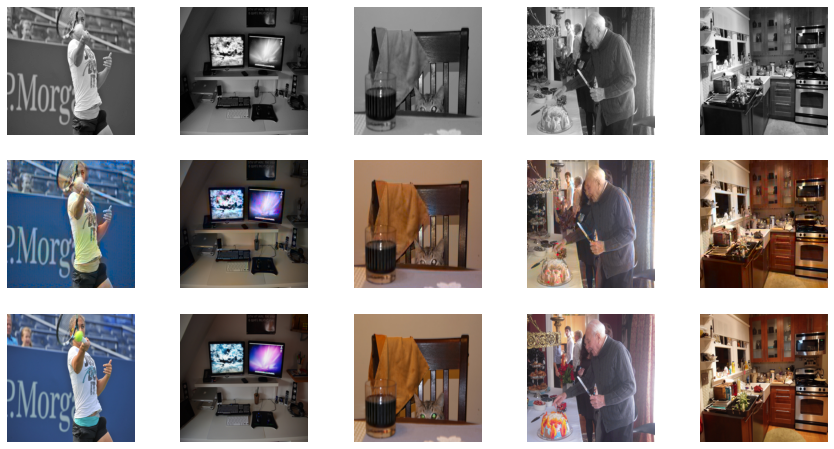
\includegraphics{Project_files/Project_62_1.png}
\caption{COCO images from the validation set colorized with the final
ViT-LSGAN model. Top row: inputs, Middle row: predictions, Bottom row:
ground truth.}
\label{fig:ViT-LSGAN-results-coco}
\end{figure}

\begin{table}\centering\caption[Metrics of the ViT-LSGAN model on validation dataset]{ViT metrics on validation dataset}\label{table:ViT-LSGAN-metrics}\begin{tabular}{llll}\toprule{}                 Metric &              a-channel &             b-channel \\\midrule               R-square &      0.9856 &     0.8596 \\     Explained variance &     0.9859 &    0.8620 \\    Mean absolute error &   0.0157 &   0.0625 \\Median absolute error &   0.0075 &   0.0374 \\Mean squared error &  0.0010 &  0.0095 \\Sample size &                   2000 &                  2000 \\\bottomrule\end{tabular}\end{table}

\hypertarget{final-colorization-results}{%
\subsection{Final colorization
results}\label{final-colorization-results}}

We tested our ViT-LSGAN with historic black and white urban pictures as
well as with historic portraits (Figures \ref{fig:Montevideo} and \ref{fig:portraits}). We noticed that sometimes old
photographs are saturated, particularly, in the sky area. This causes
the LSGAN to interpret them as cloudy skies and producing a white sky.
This effect can be partially overcome by adjusting the gain of the
original photo before feeding it into the network.

\begin{figure}
\centering
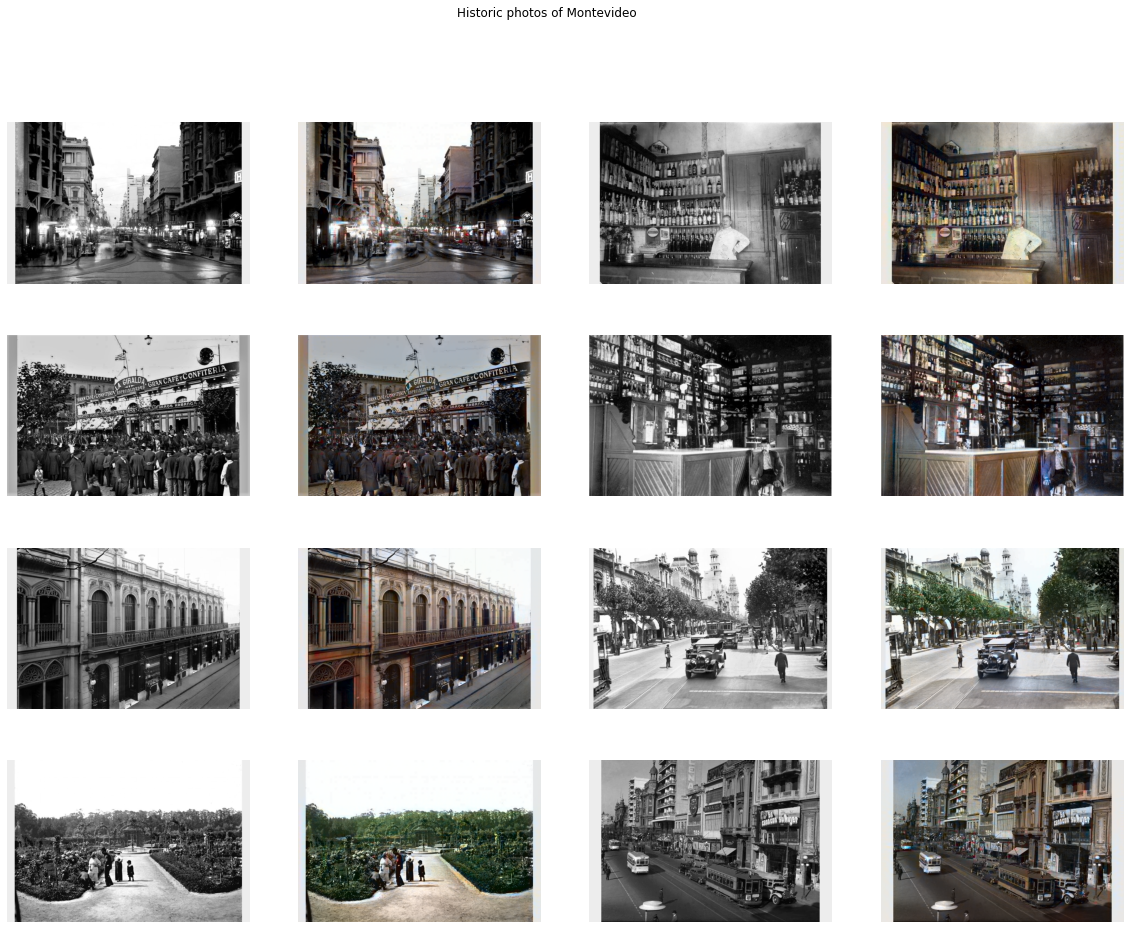
\includegraphics{Project_files/Project_72_0.png}
\caption{Historic photos of Montevideo.}
\label{fig:Montevideo}
\end{figure}

\begin{figure}
\centering
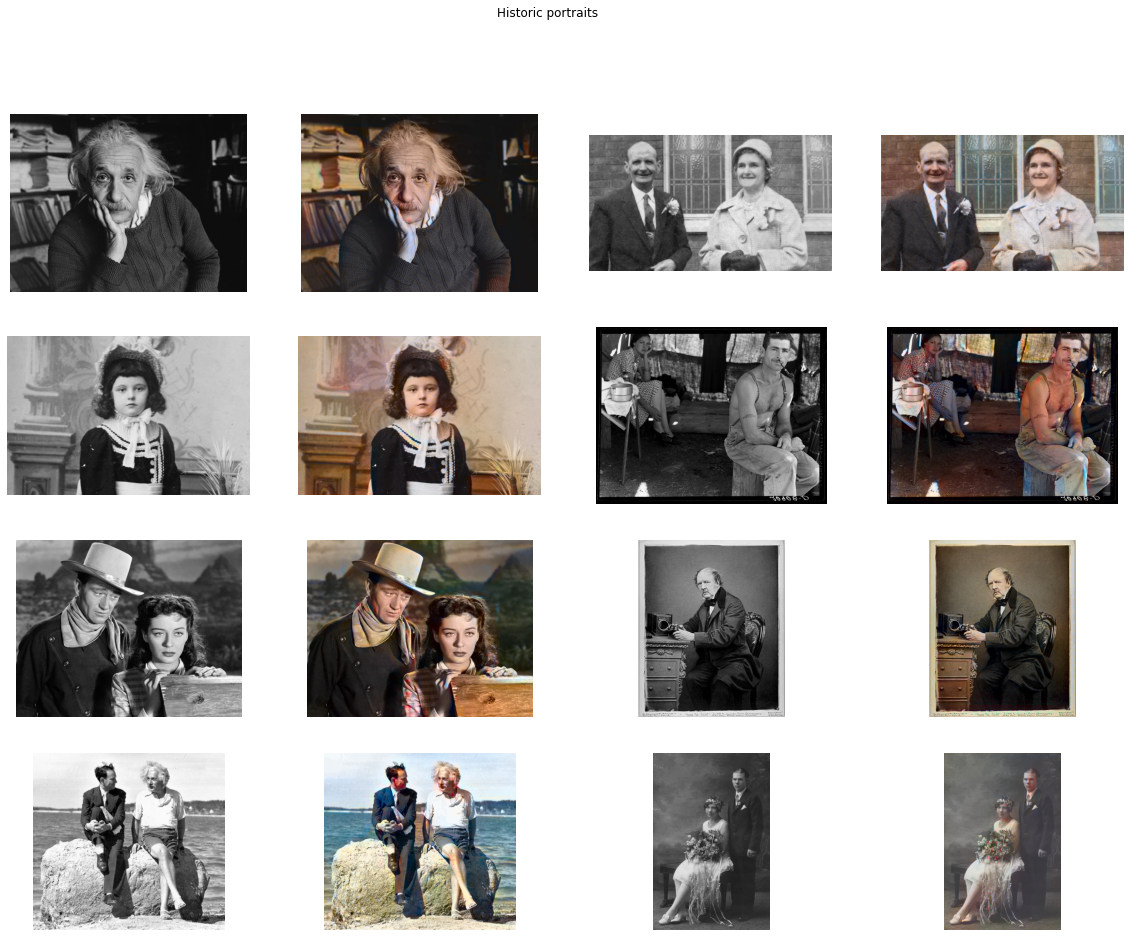
\includegraphics{Project_files/Project_73_0.png}
\caption{Historic portraits.}
\label{fig:portraits}
\end{figure}

\hypertarget{segmentation-and-blending}{%
\subsection{Segmentation and blending}\label{segmentation-and-blending}}

After colorizing the images, we segmented the foreground from the
background using the DeepLabv3 network. To obtain the final images we
blended the colorized foreground with the original black and white
background (Figures \ref{fig:segmentation-and-blending-1}-\ref{fig:segmentation-and-blending-7}).

\begin{figure}
\centering
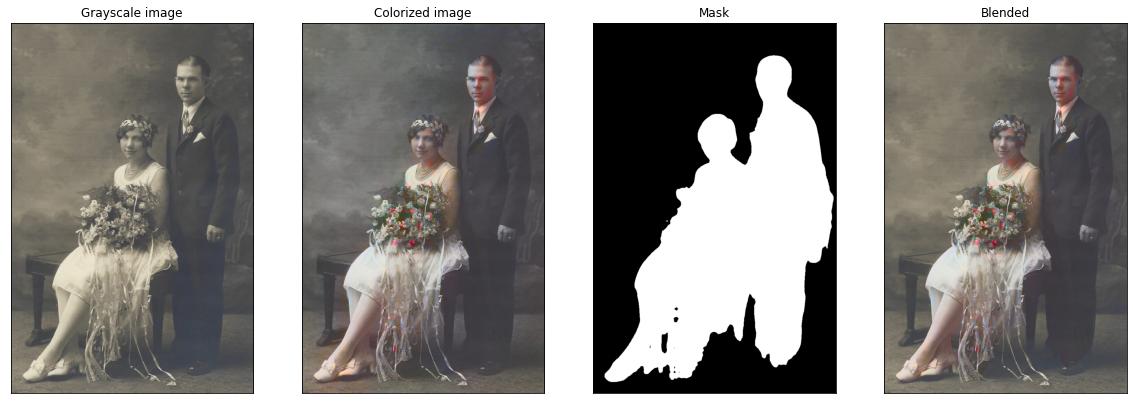
\includegraphics{report_images/segment-blend-result-7.png}
\caption{Recolorization and segmentation example 1.}
\label{fig:segmentation-and-blending-1}
\end{figure}

\begin{figure}
\centering
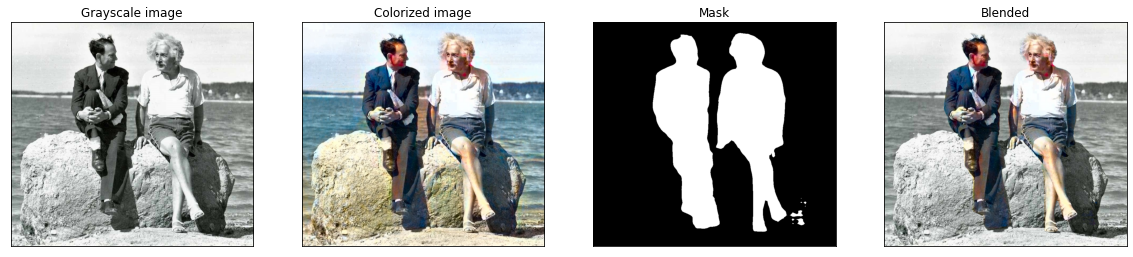
\includegraphics{report_images/segment-blend-result-6.png}
\caption{Recolorization and segmentation example 2.}
\label{fig:segmentation-and-blending-2}
\end{figure}

\begin{figure}
\centering
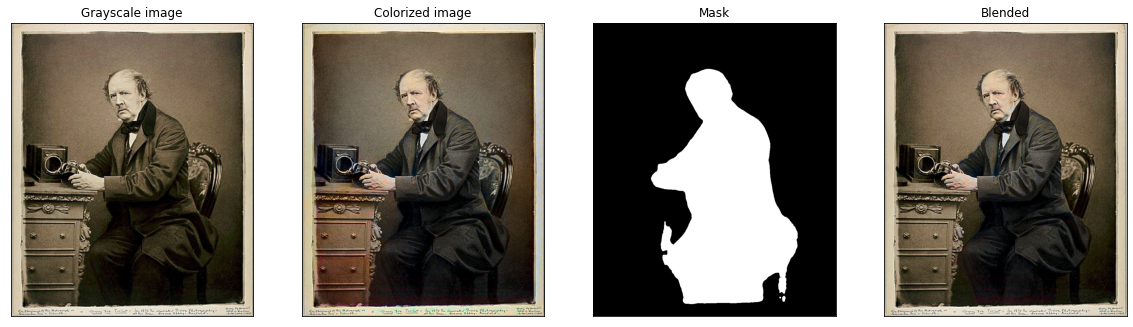
\includegraphics{report_images/segment-blend-result-5.png}
\caption{Recolorization and segmentation example 3.}
\label{fig:segmentation-and-blending-3}
\end{figure}

\begin{figure}
\centering
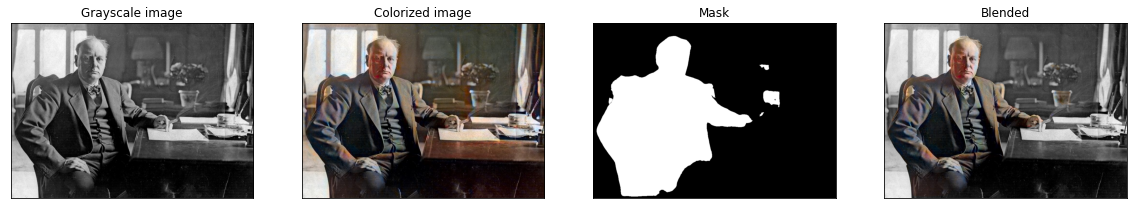
\includegraphics{report_images/segment-blend-result-4.png}
\caption{Recolorization and segmentation example 4.}
\label{fig:segmentation-and-blending-4}
\end{figure}

\begin{figure}
\centering
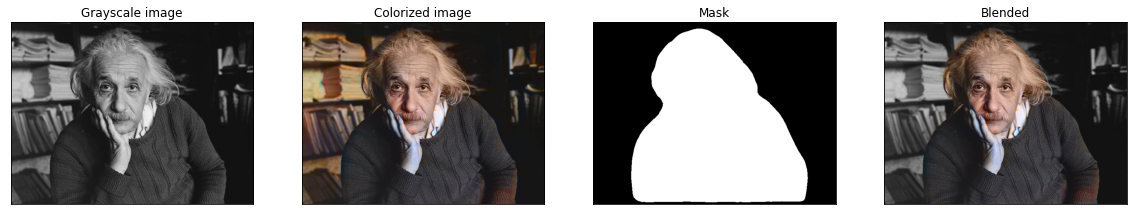
\includegraphics{report_images/segment-blend-result-3.png}
\caption{Recolorization and segmentation example 5.}
\label{fig:segmentation-and-blending-5}
\end{figure}

\begin{figure}
\centering
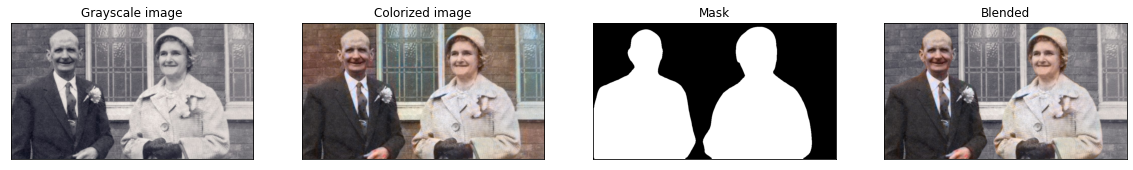
\includegraphics{report_images/segment-blend-result-2.png}
\caption{Recolorization and segmentation example 6.}
\label{fig:segmentation-and-blending-6}
\end{figure}

\begin{figure}
\centering
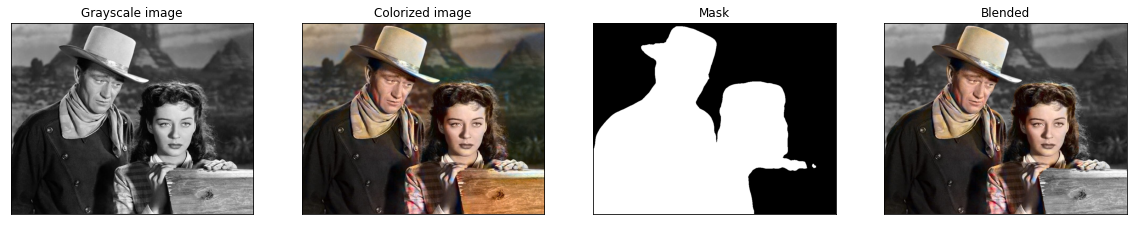
\includegraphics{report_images/segment-blend-result-1.png}
\caption{Recolorization and segmentation example 7.}
\label{fig:segmentation-and-blending-7}
\end{figure}

\begin{center}\rule{0.5\linewidth}{0.5pt}\end{center}
\clearpage
\hypertarget{supplemental-materials}{%
\section{Supplemental Materials}\label{supplemental-materials}}

\hypertarget{colorization-models-trained-and-tested}{%
\subsection{Colorization models trained and
tested}\label{colorization-models-trained-and-tested}}

\hypertarget{first-approach-resnet18-generator}{%
\subsubsection{\texorpdfstring{First approach: \emph{ResNet18}
generator}{First approach: ResNet18 generator}}\label{first-approach-resnet18-generator}}

On our first approach we employed a generator based on the ResNet18
network. One of the challenges of GANs is that, at the beginning of the
training, the task of the discriminator is much easier than that of the
generator because the generated outputs are very different from the real
ones. In this situation, the discriminator learns so much faster and
gives no time to the generator to adapt. To avoid this, we gave the
generator a \emph{head start} by training it alone (without the
generator) for 20 epochs with a L1 loss function and saving its weights.
After that we started the parallel training of the generator and the
patch discriminator for another 20 epochs (see Figure \ref{fig:resnet18} for results).

\hypertarget{second-approach-vit-as-discriminator}{%
\subsubsection{Second approach: ViT as
discriminator}\label{second-approach-vit-as-discriminator}}

Since the results obtained from the UNet generator did not look quite
natural, our first intention was to improve the discriminator so that it
will be better at telling apart the \emph{real} from the \emph{fake}
images. To do that we decided to replace the CNN based Patch
Discriminator with a Visual Transformer.

\begin{figure}
\centering
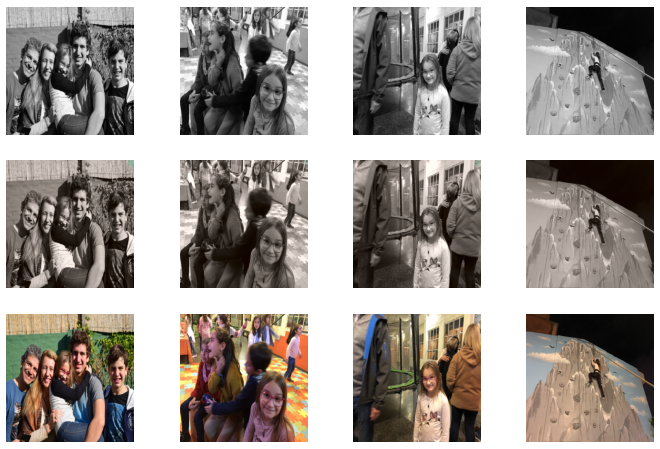
\includegraphics{results/ViTasDiscriminator.png}
\caption{Samples of results from using a ViT as the discriminator
network. Top row: inputs, Middle row: predictions, Bottom row: ground
truth.}
\label{fig:ViT-discriminator-results}
\end{figure}

Unfortunately, the results were not satisfactory (Figure \ref{fig:ViT-discriminator-results}). The discriminator got
very good a discriminating real from fake very early on and gave not
chance for the generator to adapt. The final results are just gray
images or sepia looking images with almost no color. This is because the
best loss the generator could achieve was by producing an average value
on the \textbf{ab} channels disregarding of the inputs.

\hypertarget{third-approach-vit-as-generator}{%
\subsubsection{Third approach: ViT as
generator}\label{third-approach-vit-as-generator}}

Once we understood that to have a truly creative network we should put
our efforts on the generator instead the discriminator. We decided to
include a ViT as the generator. After exploring different options we
selected a ViT trained in the task of completing masked images (Xie et
al., 2021). Since this model expects a 3-channels input, we mimicked it
just by copying the \textbf{L} channel into each of the input channels.
We replaced the decoder block of this model by 3 convolution layers and
activation functions. These layers converted the 14x14x768 inputs of the
encoder into 14x14x512 outputs. A pixel shuffle layer with an upscale
factor of 16 reshaped those outputs into the final 224x224x2 output. To
avoid the problem of the discriminator learning too fast, we kept the
pretraining step with the generator alone to give a \emph{head start} to
it. We trained for 20 epochs.

\begin{Shaded}
\begin{Highlighting}[]
\CommentTok{\# Build transformer based generator}
\CommentTok{\# https://huggingface.co/docs/transformers/model\_doc/vit}

\ImportTok{from}\NormalTok{ transformers }\ImportTok{import}\NormalTok{ ViTForMaskedImageModeling, ViTConfig}


\KeywordTok{def}\NormalTok{ build\_VTi\_generator():}

    \CommentTok{\#\# Pretrained generator ViT, 3{-}input channels, multilayer decoder.}
\NormalTok{    device }\OperatorTok{=}\NormalTok{ torch.device(}\StringTok{"cuda"} \ControlFlowTok{if}\NormalTok{ torch.cuda.is\_available() }\ControlFlowTok{else} \StringTok{"cpu"}\NormalTok{)}
\NormalTok{    model }\OperatorTok{=}\NormalTok{ ViTForMaskedImageModeling.from\_pretrained(}\StringTok{"google/vit{-}base{-}patch16{-}224{-}in21k"}\NormalTok{)}

\NormalTok{    model.decoder }\OperatorTok{=}\NormalTok{ nn.Sequential(nn.Conv2d(}\DecValTok{768}\NormalTok{, }\DecValTok{768}\NormalTok{, kernel\_size}\OperatorTok{=}\DecValTok{3}\NormalTok{, stride}\OperatorTok{=}\DecValTok{1}\NormalTok{, padding}\OperatorTok{=}\DecValTok{1}\NormalTok{), }\OperatorTok{\textbackslash{}}
\NormalTok{                                    nn.ReLU(inplace}\OperatorTok{=}\VariableTok{True}\NormalTok{),}
\NormalTok{                                    nn.Conv2d(}\DecValTok{768}\NormalTok{, }\DecValTok{768}\NormalTok{, kernel\_size}\OperatorTok{=}\DecValTok{3}\NormalTok{, stride}\OperatorTok{=}\DecValTok{1}\NormalTok{, padding}\OperatorTok{=}\DecValTok{1}\NormalTok{), }\OperatorTok{\textbackslash{}}
\NormalTok{                                    nn.ReLU(inplace}\OperatorTok{=}\VariableTok{True}\NormalTok{),}
\NormalTok{                                    nn.Conv2d(}\DecValTok{768}\NormalTok{, }\DecValTok{512}\NormalTok{, kernel\_size}\OperatorTok{=}\DecValTok{3}\NormalTok{, stride}\OperatorTok{=}\DecValTok{1}\NormalTok{, padding}\OperatorTok{=}\DecValTok{1}\NormalTok{), }\OperatorTok{\textbackslash{}}
\NormalTok{                                    nn.PixelShuffle(upscale\_factor}\OperatorTok{=}\DecValTok{16}\NormalTok{))}
\NormalTok{    model }\OperatorTok{=}\NormalTok{ model.to(device)}
    \ControlFlowTok{return}\NormalTok{ model}
\end{Highlighting}
\end{Shaded}

\begin{figure}
\centering
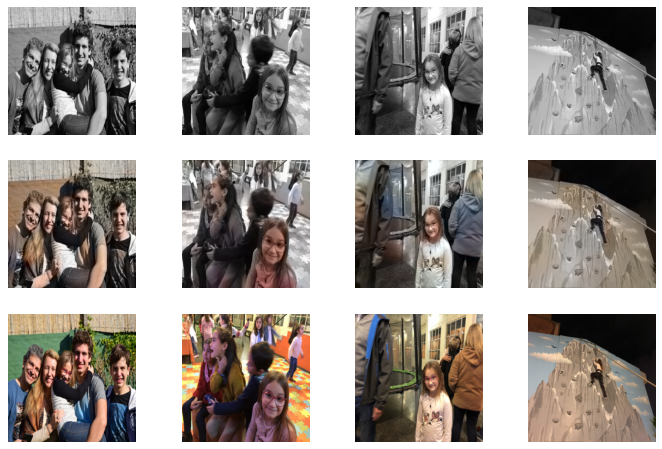
\includegraphics{results/Pretrained3channelViT_task_pretraining_result.png}
\caption{Samples of results from pretraining the ViT generator alone.
Top row: inputs, Middle row: predictions, Bottom row: ground truth.}
\label{fig:pretraining-ViT-results}
\end{figure}

\begin{figure}
\centering
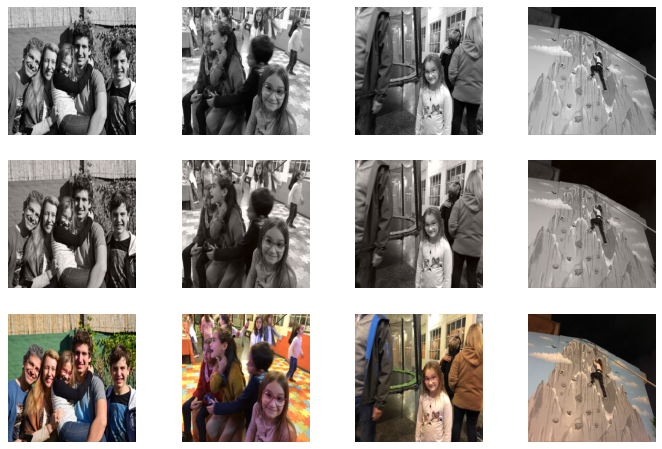
\includegraphics{results/Pretrained3channelViT_task_pretraining_FINAL_result.png}
\caption{Samples of results after training the ViT generator with the
discriminator. Top row: inputs, Middle row: predictions, Bottom row:
ground truth.}
\label{fig:ViT-pretrained-results}
\end{figure}

The results were not very encouraging. After the pretraining when the
generator trained alone, the results were acceptable although the colors
were not very bright or varied (Figure \ref{fig:pretraining-ViT-results}). However, when we trained with the
discriminator, the discriminator won the game and the generator produced
just gray images, as before (Figure \ref{fig:ViT-pretrained-results}).

\hypertarget{fourth-approach-lsgan-with-vit}{%
\subsubsection{Fourth approach: LSGAN with
ViT}\label{fourth-approach-lsgan-with-vit}}

The other main challenge of training a GAN is choosing the right loss
function. During training of regular networks a convergence of the loss
function to a small enough value signals that the network has achieved
an equilibrium and cannot learn more from the training data. However,
training of a GAN is a two players game in which each one tries to
minimize its own loss by maximizing the other player loss. The generator
and discriminator losses should not converge but stay in a permanent
unstable equilibrium which signals that the game is still being played.

The loss function is what gives the gradient the generator needs to
learn to fool the discriminator and not all loss functions are equal for
this task. As already mentioned, at the beginning of the training it is
very easy for the discriminator to tell fake from real. When Cross
Entropy is used, it can provide very low or vanishing gradients at the
start of the training that do not help the improvement of the generator.
To overcome this problem, it has been suggested the use of least squared
errors loss functions (Mao et al., 2016). Therefore, we replaced the BCE
loss with least square errors loss to construct a \textbf{ViT-LSGAN}.
This architecture gave the best results. The results and metrics
obtained with this model were presented before (Figures \ref{fig:ViT-LSGAN-results} and \ref{fig:ViT-LSGAN-results-coco}, Table \ref{table:ViT-LSGAN-metrics}).

\hypertarget{image-upscaling}{%
\subsection{Image Upscaling}\label{image-upscaling}}

The ViT-LSGAN was trained with 224 by 224 images, so it is better to use
downsampled images for transfering color. To colorize the full size
image, we upscaled the outputs of the network by resizing the predicted
\textbf{ab} channels to the size of the original \textbf{L} channel, and
combined the results with the \textbf{L} channel to produce a color
image in the \textbf{Lab} colorspace.

\clearpage
\hypertarget{selected-python-code-sections}{%
\subsection{Selected Python code
sections}\label{selected-python-code-sections}}

\hypertarget{colorization-model-class}{%
\subsubsection{Colorization Model
class}\label{colorization-model-class}}

\begin{Shaded}
\begin{Highlighting}[]
\KeywordTok{class}\NormalTok{ MainModel(nn.Module):}
    \KeywordTok{def} \FunctionTok{\_\_init\_\_}\NormalTok{(}\VariableTok{self}\NormalTok{, net\_G}\OperatorTok{=}\VariableTok{None}\NormalTok{, net\_D}\OperatorTok{=}\VariableTok{None}\NormalTok{, use\_ViT\_gen }\OperatorTok{=} \VariableTok{False}\NormalTok{, lr\_G}\OperatorTok{=}\FloatTok{2e{-}4}\NormalTok{, lr\_D}\OperatorTok{=}\FloatTok{2e{-}4}\NormalTok{, }
\NormalTok{                 beta1}\OperatorTok{=}\FloatTok{0.5}\NormalTok{, beta2}\OperatorTok{=}\FloatTok{0.999}\NormalTok{, lambda\_L1}\OperatorTok{=}\FloatTok{100.}\NormalTok{):}
        \BuiltInTok{super}\NormalTok{().}\FunctionTok{\_\_init\_\_}\NormalTok{()}
        
        \VariableTok{self}\NormalTok{.device }\OperatorTok{=}\NormalTok{ torch.device(}\StringTok{"cuda"} \ControlFlowTok{if}\NormalTok{ torch.cuda.is\_available() }\ControlFlowTok{else} \StringTok{"cpu"}\NormalTok{)}
        \VariableTok{self}\NormalTok{.lambda\_L1 }\OperatorTok{=}\NormalTok{ lambda\_L1}
        \VariableTok{self}\NormalTok{.use\_ViT\_gen }\OperatorTok{=}\NormalTok{ use\_ViT\_gen}
        
        \ControlFlowTok{if}\NormalTok{ net\_G }\KeywordTok{is} \VariableTok{None}\NormalTok{:}
            \ControlFlowTok{raise} \PreprocessorTok{NotImplementedError}
        \ControlFlowTok{else}\NormalTok{:}
            \VariableTok{self}\NormalTok{.net\_G }\OperatorTok{=}\NormalTok{ net\_G.to(}\VariableTok{self}\NormalTok{.device)}
        
        \ControlFlowTok{if}\NormalTok{ net\_D }\KeywordTok{is} \VariableTok{None}\NormalTok{:}
            \VariableTok{self}\NormalTok{.net\_D }\OperatorTok{=}\NormalTok{ init\_model(PatchDiscriminator(input\_c}\OperatorTok{=}\DecValTok{3}\NormalTok{, n\_down}\OperatorTok{=}\DecValTok{3}\NormalTok{, num\_filters}\OperatorTok{=}\DecValTok{64}\NormalTok{), }\VariableTok{self}\NormalTok{.device)}
        \ControlFlowTok{else}\NormalTok{:}
            \VariableTok{self}\NormalTok{.net\_D }\OperatorTok{=}\NormalTok{ net\_D.to(}\VariableTok{self}\NormalTok{.device)}
            
        \CommentTok{\#self.GANcriterion = GANLoss(gan\_mode=\textquotesingle{}vanilla\textquotesingle{}).to(self.device)  \# Original BCE Loss}
        \VariableTok{self}\NormalTok{.GANcriterion }\OperatorTok{=}\NormalTok{ GANLoss(gan\_mode}\OperatorTok{=}\StringTok{\textquotesingle{}lsgan\textquotesingle{}}\NormalTok{).to(}\VariableTok{self}\NormalTok{.device)  }\CommentTok{\# Final improvement with Least Square Error loss}
        \VariableTok{self}\NormalTok{.L1criterion }\OperatorTok{=}\NormalTok{ nn.L1Loss()}
        \VariableTok{self}\NormalTok{.opt\_G }\OperatorTok{=}\NormalTok{ optim.Adam(}\VariableTok{self}\NormalTok{.net\_G.parameters(), lr}\OperatorTok{=}\NormalTok{lr\_G, betas}\OperatorTok{=}\NormalTok{(beta1, beta2))}
        \VariableTok{self}\NormalTok{.opt\_D }\OperatorTok{=}\NormalTok{ optim.Adam(}\VariableTok{self}\NormalTok{.net\_D.parameters(), lr}\OperatorTok{=}\NormalTok{lr\_D, betas}\OperatorTok{=}\NormalTok{(beta1, beta2))}
    
    \KeywordTok{def}\NormalTok{ set\_requires\_grad(}\VariableTok{self}\NormalTok{, model, requires\_grad}\OperatorTok{=}\VariableTok{True}\NormalTok{):}
        \ControlFlowTok{for}\NormalTok{ p }\KeywordTok{in}\NormalTok{ model.parameters():}
\NormalTok{            p.requires\_grad }\OperatorTok{=}\NormalTok{ requires\_grad}
        
    \KeywordTok{def}\NormalTok{ setup\_input(}\VariableTok{self}\NormalTok{, data):}
        \VariableTok{self}\NormalTok{.L }\OperatorTok{=}\NormalTok{ data[}\StringTok{\textquotesingle{}L\textquotesingle{}}\NormalTok{].to(}\VariableTok{self}\NormalTok{.device)}
        \VariableTok{self}\NormalTok{.ab }\OperatorTok{=}\NormalTok{ data[}\StringTok{\textquotesingle{}ab\textquotesingle{}}\NormalTok{].to(}\VariableTok{self}\NormalTok{.device)}
        
    \KeywordTok{def}\NormalTok{ forward(}\VariableTok{self}\NormalTok{):}
        \ControlFlowTok{if}\NormalTok{ (}\VariableTok{self}\NormalTok{.use\_ViT\_gen }\OperatorTok{==} \VariableTok{True}\NormalTok{):}
\NormalTok{            outputs }\OperatorTok{=} \VariableTok{self}\NormalTok{.net\_G(}\VariableTok{self}\NormalTok{.L.repeat(}\DecValTok{1}\NormalTok{,}\DecValTok{3}\NormalTok{,}\DecValTok{1}\NormalTok{,}\DecValTok{1}\NormalTok{))  }\CommentTok{\# Copy the L channel 3 times to mimick the 3{-}channels input that the pretrained network requires.}
            \VariableTok{self}\NormalTok{.fake\_color }\OperatorTok{=}\NormalTok{ outputs.logits}
        \ControlFlowTok{else}\NormalTok{:}
            \VariableTok{self}\NormalTok{.fake\_color }\OperatorTok{=} \VariableTok{self}\NormalTok{.net\_G(}\VariableTok{self}\NormalTok{.L)}
    
    \KeywordTok{def}\NormalTok{ backward\_D(}\VariableTok{self}\NormalTok{):}
\NormalTok{        fake\_image }\OperatorTok{=}\NormalTok{ torch.cat([}\VariableTok{self}\NormalTok{.L, }\VariableTok{self}\NormalTok{.fake\_color], dim}\OperatorTok{=}\DecValTok{1}\NormalTok{)}
\NormalTok{        fake\_preds }\OperatorTok{=} \VariableTok{self}\NormalTok{.net\_D(fake\_image.detach())}
        \VariableTok{self}\NormalTok{.loss\_D\_fake }\OperatorTok{=} \VariableTok{self}\NormalTok{.GANcriterion(fake\_preds, }\VariableTok{False}\NormalTok{)}
\NormalTok{        real\_image }\OperatorTok{=}\NormalTok{ torch.cat([}\VariableTok{self}\NormalTok{.L, }\VariableTok{self}\NormalTok{.ab], dim}\OperatorTok{=}\DecValTok{1}\NormalTok{)}
\NormalTok{        real\_preds }\OperatorTok{=} \VariableTok{self}\NormalTok{.net\_D(real\_image)}
        \VariableTok{self}\NormalTok{.loss\_D\_real }\OperatorTok{=} \VariableTok{self}\NormalTok{.GANcriterion(real\_preds, }\VariableTok{True}\NormalTok{)}
        \VariableTok{self}\NormalTok{.loss\_D }\OperatorTok{=}\NormalTok{ (}\VariableTok{self}\NormalTok{.loss\_D\_fake }\OperatorTok{+} \VariableTok{self}\NormalTok{.loss\_D\_real) }\OperatorTok{*} \FloatTok{0.5}
        \VariableTok{self}\NormalTok{.loss\_D.backward()}
        
    \KeywordTok{def}\NormalTok{ backward\_G(}\VariableTok{self}\NormalTok{):}
\NormalTok{        fake\_image }\OperatorTok{=}\NormalTok{ torch.cat([}\VariableTok{self}\NormalTok{.L, }\VariableTok{self}\NormalTok{.fake\_color], dim}\OperatorTok{=}\DecValTok{1}\NormalTok{)}
\NormalTok{        fake\_preds }\OperatorTok{=} \VariableTok{self}\NormalTok{.net\_D(fake\_image)}
        \VariableTok{self}\NormalTok{.loss\_G\_GAN }\OperatorTok{=} \VariableTok{self}\NormalTok{.GANcriterion(fake\_preds, }\VariableTok{True}\NormalTok{)}
        \VariableTok{self}\NormalTok{.loss\_G\_L1 }\OperatorTok{=} \VariableTok{self}\NormalTok{.L1criterion(}\VariableTok{self}\NormalTok{.fake\_color, }\VariableTok{self}\NormalTok{.ab) }\OperatorTok{*} \VariableTok{self}\NormalTok{.lambda\_L1}
        \VariableTok{self}\NormalTok{.loss\_G }\OperatorTok{=} \VariableTok{self}\NormalTok{.loss\_G\_GAN }\OperatorTok{+} \VariableTok{self}\NormalTok{.loss\_G\_L1}
        \VariableTok{self}\NormalTok{.loss\_G.backward()}
    
    \KeywordTok{def}\NormalTok{ optimize(}\VariableTok{self}\NormalTok{):}
        \VariableTok{self}\NormalTok{.forward()}
        \VariableTok{self}\NormalTok{.net\_D.train()}
        \VariableTok{self}\NormalTok{.set\_requires\_grad(}\VariableTok{self}\NormalTok{.net\_D, }\VariableTok{True}\NormalTok{)}
        \VariableTok{self}\NormalTok{.opt\_D.zero\_grad()}
        \VariableTok{self}\NormalTok{.backward\_D()}
        \VariableTok{self}\NormalTok{.opt\_D.step()}
        
        \VariableTok{self}\NormalTok{.net\_G.train()}
        \VariableTok{self}\NormalTok{.set\_requires\_grad(}\VariableTok{self}\NormalTok{.net\_D, }\VariableTok{False}\NormalTok{)}
        \VariableTok{self}\NormalTok{.opt\_G.zero\_grad()}
        \VariableTok{self}\NormalTok{.backward\_G()}
        \VariableTok{self}\NormalTok{.opt\_G.step()}
\end{Highlighting}
\end{Shaded}
\clearpage
\hypertarget{deeplabv3-based-segmentation}{%
\subsubsection{DeepLabv3 based
segmentation}\label{deeplabv3-based-segmentation}}

\begin{Shaded}
\begin{Highlighting}[]
\ImportTok{from}\NormalTok{ torchvision }\ImportTok{import}\NormalTok{ models}
\ImportTok{import}\NormalTok{ torchvision.transforms }\ImportTok{as}\NormalTok{ T}
\ImportTok{import}\NormalTok{ torch}
\ImportTok{import}\NormalTok{ cv2}
\ImportTok{import}\NormalTok{ numpy }\ImportTok{as}\NormalTok{ np}
\ImportTok{from}\NormalTok{ PIL }\ImportTok{import}\NormalTok{ Image}
\ImportTok{import}\NormalTok{ matplotlib.pyplot }\ImportTok{as}\NormalTok{ plt}

\NormalTok{dlv3 }\OperatorTok{=}\NormalTok{ models.segmentation.deeplabv3\_resnet101(pretrained}\OperatorTok{=}\DecValTok{1}\NormalTok{).}\BuiltInTok{eval}\NormalTok{()}
\NormalTok{n\_classes }\OperatorTok{=} \DecValTok{21} 
\NormalTok{palette }\OperatorTok{=}\NormalTok{ torch.tensor([}\DecValTok{2} \OperatorTok{**} \DecValTok{25} \OperatorTok{{-}} \DecValTok{1}\NormalTok{, }\DecValTok{2} \OperatorTok{**} \DecValTok{15} \OperatorTok{{-}} \DecValTok{1}\NormalTok{, }\DecValTok{2} \OperatorTok{**} \DecValTok{21} \OperatorTok{{-}} \DecValTok{1}\NormalTok{])}
\NormalTok{colors }\OperatorTok{=}\NormalTok{ torch.as\_tensor([i }\ControlFlowTok{for}\NormalTok{ i }\KeywordTok{in} \BuiltInTok{range}\NormalTok{(n\_classes)])[:, }\VariableTok{None}\NormalTok{] }\OperatorTok{*}\NormalTok{ palette}

\NormalTok{grayscale\_images }\OperatorTok{=}\NormalTok{ (}
\NormalTok{    imgs\_grayscale\_1,}
\NormalTok{    imgs\_grayscale\_2,}
\NormalTok{    imgs\_grayscale\_3,}
\NormalTok{    imgs\_grayscale\_4,}
\NormalTok{    imgs\_grayscale\_5,}
\NormalTok{    imgs\_grayscale\_6,}
\NormalTok{    imgs\_grayscale\_7,}
\NormalTok{    imgs\_grayscale\_8,}
\NormalTok{)}


\NormalTok{colorized\_images }\OperatorTok{=}\NormalTok{ (}
\NormalTok{    imgs\_color\_1,}
\NormalTok{    imgs\_color\_2,}
\NormalTok{    imgs\_color\_3,}
\NormalTok{    imgs\_color\_4,}
\NormalTok{    imgs\_color\_5,}
\NormalTok{    imgs\_color\_6,}
\NormalTok{    imgs\_color\_7,}
\NormalTok{    imgs\_color\_8,}
\NormalTok{)}

\KeywordTok{def}\NormalTok{ infer\_segment\_color(img):}
\NormalTok{  [r,g,b] }\OperatorTok{=} \DecValTok{3} \OperatorTok{*}\NormalTok{ [np.zeros\_like(img).astype(np.uint8)]}
  \ControlFlowTok{for}\NormalTok{ i }\KeywordTok{in} \BuiltInTok{range}\NormalTok{(n\_classes):}
\NormalTok{    idx }\OperatorTok{=}\NormalTok{ (img }\OperatorTok{==}\NormalTok{ i)}
\NormalTok{    r[idx],  g[idx],  b[idx] }\OperatorTok{=}\NormalTok{  colors[i, }\DecValTok{0}\NormalTok{],  colors[i, }\DecValTok{1}\NormalTok{], colors[i, }\DecValTok{2}\NormalTok{]}
\NormalTok{  rgb }\OperatorTok{=}\NormalTok{ np.stack([r, g, b], axis}\OperatorTok{=}\DecValTok{2}\NormalTok{)}
  \ControlFlowTok{return}\NormalTok{ rgb}

\KeywordTok{def}\NormalTok{ generate\_mask(img):}
\NormalTok{  transform }\OperatorTok{=}\NormalTok{ T.Compose([}
\NormalTok{                     T.ToTensor(),}
\NormalTok{                     T.Normalize(mean }\OperatorTok{=}\NormalTok{ [}\FloatTok{0.485}\NormalTok{, }\FloatTok{0.456}\NormalTok{, }\FloatTok{0.406}\NormalTok{],  std }\OperatorTok{=}\NormalTok{ [}\FloatTok{0.229}\NormalTok{, }\FloatTok{0.224}\NormalTok{, }\FloatTok{0.225}\NormalTok{])])}
\NormalTok{  output }\OperatorTok{=}\NormalTok{ dlv3(transform(img).unsqueeze(}\DecValTok{0}\NormalTok{))[}\StringTok{\textquotesingle{}out\textquotesingle{}}\NormalTok{]}
\NormalTok{  mask }\OperatorTok{=}\NormalTok{ torch.argmax(output.squeeze(), dim}\OperatorTok{=}\DecValTok{0}\NormalTok{).detach().cpu().numpy()}
\NormalTok{  mask }\OperatorTok{=}\NormalTok{ infer\_segment\_color(mask)}
  \BuiltInTok{print}\NormalTok{(}\StringTok{"Mask shape"}\NormalTok{, mask.shape)}
  \ControlFlowTok{return}\NormalTok{ mask}

\NormalTok{masks }\OperatorTok{=}\NormalTok{ \{\} }
\NormalTok{masks[}\DecValTok{0}\NormalTok{] }\OperatorTok{=}\NormalTok{ generate\_mask(imgs\_grayscale\_1)}
\NormalTok{masks[}\DecValTok{1}\NormalTok{] }\OperatorTok{=}\NormalTok{ generate\_mask(imgs\_grayscale\_2)}
\NormalTok{masks[}\DecValTok{2}\NormalTok{] }\OperatorTok{=}\NormalTok{ generate\_mask(imgs\_grayscale\_3)}
\NormalTok{masks[}\DecValTok{3}\NormalTok{] }\OperatorTok{=}\NormalTok{ generate\_mask(imgs\_grayscale\_4)}
\NormalTok{masks[}\DecValTok{4}\NormalTok{] }\OperatorTok{=}\NormalTok{ generate\_mask(imgs\_grayscale\_5)}
\NormalTok{masks[}\DecValTok{5}\NormalTok{] }\OperatorTok{=}\NormalTok{ generate\_mask(imgs\_grayscale\_6)}
\NormalTok{masks[}\DecValTok{6}\NormalTok{] }\OperatorTok{=}\NormalTok{ generate\_mask(imgs\_grayscale\_7)}
\NormalTok{masks[}\DecValTok{7}\NormalTok{] }\OperatorTok{=}\NormalTok{ generate\_mask(imgs\_grayscale\_8)}

\NormalTok{\_masks }\OperatorTok{=}\NormalTok{ []}
\NormalTok{\_reverse\_masks }\OperatorTok{=}\NormalTok{ []}
\NormalTok{blended\_images }\OperatorTok{=}\NormalTok{ []}

\ControlFlowTok{for}\NormalTok{ i }\KeywordTok{in} \BuiltInTok{range}\NormalTok{(}\BuiltInTok{len}\NormalTok{(masks)):}
\NormalTok{    \_mask }\OperatorTok{=}\NormalTok{ ((masks[i] }\OperatorTok{!=} \DecValTok{0}\NormalTok{).astype(}\BuiltInTok{int}\NormalTok{))}
\NormalTok{    \_masks.append(\_mask)}
\NormalTok{    \_rev\_mask }\OperatorTok{=}\NormalTok{  ( (masks[i] }\OperatorTok{==} \DecValTok{0}\NormalTok{).astype(}\BuiltInTok{int}\NormalTok{))}
\NormalTok{    \_reverse\_masks.append(\_rev\_mask)}
\NormalTok{    blended\_images.append(\_mask }\OperatorTok{*}\NormalTok{ colorized\_images[i] }\OperatorTok{+}\NormalTok{ \_rev\_mask }\OperatorTok{*}\NormalTok{ grayscale\_images[i])}
    
\KeywordTok{def}\NormalTok{ show\_images(im\_grayscale, im\_colorized, im\_mask, im\_blended):}
\NormalTok{    fig, axes }\OperatorTok{=}\NormalTok{ plt.subplots(}\DecValTok{1}\NormalTok{, }\DecValTok{4}\NormalTok{, figsize}\OperatorTok{=}\NormalTok{(}\DecValTok{20}\NormalTok{,}\DecValTok{20}\NormalTok{))}
\NormalTok{    axes[}\DecValTok{0}\NormalTok{].imshow(im\_grayscale, cmap}\OperatorTok{=}\StringTok{\textquotesingle{}gray\textquotesingle{}}\NormalTok{)}
\NormalTok{    axes[}\DecValTok{0}\NormalTok{].set\_title(}\StringTok{\textquotesingle{}Grayscale image\textquotesingle{}}\NormalTok{), axes[}\DecValTok{0}\NormalTok{].set\_xticks([]), axes[}\DecValTok{0}\NormalTok{].set\_yticks([])}
\NormalTok{    axes[}\DecValTok{1}\NormalTok{].imshow(im\_colorized,cmap}\OperatorTok{=}\StringTok{\textquotesingle{}gray\textquotesingle{}}\NormalTok{)}
\NormalTok{    axes[}\DecValTok{1}\NormalTok{].set\_title(}\StringTok{\textquotesingle{}Colorized image\textquotesingle{}}\NormalTok{), axes[}\DecValTok{1}\NormalTok{].set\_xticks([]), axes[}\DecValTok{1}\NormalTok{].set\_yticks([])}\OperatorTok{;}
\NormalTok{    axes[}\DecValTok{2}\NormalTok{].imshow(im\_mask }\OperatorTok{*} \DecValTok{255}\NormalTok{,cmap}\OperatorTok{=}\StringTok{\textquotesingle{}gray\textquotesingle{}}\NormalTok{)}
\NormalTok{    axes[}\DecValTok{2}\NormalTok{].set\_title(}\StringTok{\textquotesingle{}Mask\textquotesingle{}}\NormalTok{), axes[}\DecValTok{2}\NormalTok{].set\_xticks([]), axes[}\DecValTok{2}\NormalTok{].set\_yticks([])}\OperatorTok{;}
\NormalTok{    axes[}\DecValTok{3}\NormalTok{].imshow(im\_blended ,cmap}\OperatorTok{=}\StringTok{\textquotesingle{}gray\textquotesingle{}}\NormalTok{)}
\NormalTok{    axes[}\DecValTok{3}\NormalTok{].set\_title(}\StringTok{\textquotesingle{}Blended\textquotesingle{}}\NormalTok{), axes[}\DecValTok{3}\NormalTok{].set\_xticks([]), axes[}\DecValTok{3}\NormalTok{].set\_yticks([])}\OperatorTok{;}

\ControlFlowTok{for}\NormalTok{ i }\KeywordTok{in} \BuiltInTok{range}\NormalTok{(}\BuiltInTok{len}\NormalTok{(grayscale\_images)): }
\NormalTok{    show\_images(grayscale\_images[i], colorized\_images[i], \_masks[i], blended\_images[i])}
\end{Highlighting}
\end{Shaded}

\begin{center}\rule{0.5\linewidth}{0.5pt}\end{center}
\clearpage
\hypertarget{references}{%
\section*{References}\label{references}}
\addcontentsline{toc}{section}{References}

\hypertarget{refs}{}
\begin{CSLReferences}{1}{0}
\leavevmode\vadjust pre{\hypertarget{ref-7913730}{}}%
Chen, L.-C., Papandreou, G., Kokkinos, I., Murphy, K., \& Yuille, A. L.
(2018). DeepLab: Semantic image segmentation with deep convolutional
nets, atrous convolution, and fully connected CRFs. \emph{IEEE
Transactions on Pattern Analysis and Machine Intelligence},
\emph{40}(4), 834--848. \url{https://doi.org/10.1109/TPAMI.2017.2699184}

\leavevmode\vadjust pre{\hypertarget{ref-chen2017rethinking}{}}%
Chen, L.-C., Papandreou, G., Schroff, F., \& Adam, H. (2017). Rethinking
atrous convolution for semantic image segmentation. \emph{arXiv Preprint
arXiv:1706.05587}.

\leavevmode\vadjust pre{\hypertarget{ref-colorizationtutorial}{}}%
\emph{Colorizing black \& white images with u-net and conditional GAN
--- a tutorial}. (n.d.).
\url{https://towardsdatascience.com/colorizing-black-white-images-with-u-net-and-conditional-gan-a-tutorial-81b2df111cd8}.

\leavevmode\vadjust pre{\hypertarget{ref-ViT}{}}%
Dosovitskiy, A., Beyer, L., Kolesnikov, A., Weissenborn, D., Zhai, X.,
Unterthiner, T., Dehghani, M., Minderer, M., Heigold, G., Gelly, S.,
Uszkoreit, J., \& Houlsby, N. (2020). An image is worth 16x16 words:
Transformers for image recognition at scale. \emph{CoRR},
\emph{abs/2010.11929}. \url{https://arxiv.org/abs/2010.11929}

\leavevmode\vadjust pre{\hypertarget{ref-fastai}{}}%
\emph{Fast.ai}. (n.d.). \url{https://www.fast.ai/}.

\leavevmode\vadjust pre{\hypertarget{ref-goodfellow2014}{}}%
Goodfellow, I. J., Pouget-Abadie, J., Mirza, M., Xu, B., Warde-Farley,
D., Ozair, S., Courville, A., \& Bengio, Y. (2014). \emph{Generative
adversarial networks}. \url{https://doi.org/10.48550/ARXIV.1406.2661}

\leavevmode\vadjust pre{\hypertarget{ref-pix2pix}{}}%
Isola, P., Zhu, J.-Y., Zhou, T., \& Efros, A. A. (2016). Image-to-image
translation with conditional adversarial networks. \emph{CoRR},
\emph{abs/1611.07004}. \url{http://arxiv.org/abs/1611.07004}

\leavevmode\vadjust pre{\hypertarget{ref-cocodataset}{}}%
Lin, T.-Y., Maire, M., Belongie, S. J., Bourdev, L. D., Girshick, R. B.,
Hays, J., Perona, P., Ramanan, D., Dollár, P., \& Zitnick, C. L. (2014).
Microsoft {COCO:} Common objects in context. \emph{CoRR},
\emph{abs/1405.0312}. \url{http://arxiv.org/abs/1405.0312}

\leavevmode\vadjust pre{\hypertarget{ref-LSGAN}{}}%
Mao, X., Li, Q., Xie, H., Lau, R. Y. K., \& Wang, Z. (2016). Multi-class
generative adversarial networks with the {L2} loss function.
\emph{CoRR}, \emph{abs/1611.04076}.
\url{http://arxiv.org/abs/1611.04076}

\leavevmode\vadjust pre{\hypertarget{ref-transformers}{}}%
Vaswani, A., Shazeer, N., Parmar, N., Uszkoreit, J., Jones, L., Gomez,
A. N., Kaiser, L., \& Polosukhin, I. (2017). Attention is all you need.
\emph{CoRR}, \emph{abs/1706.03762}.
\url{http://arxiv.org/abs/1706.03762}

\leavevmode\vadjust pre{\hypertarget{ref-Zhenda2021}{}}%
Xie, Z., Zhang, Z., Cao, Y., Lin, Y., Bao, J., Yao, Z., Dai, Q., \& Hu,
H. (2021). SimMIM: {A} simple framework for masked image modeling.
\emph{CoRR}, \emph{abs/2111.09886}.
\url{https://arxiv.org/abs/2111.09886}

\leavevmode\vadjust pre{\hypertarget{ref-ZhangIE16}{}}%
Zhang, R., Isola, P., \& Efros, A. A. (2016). Colorful image
colorization. \emph{CoRR}, \emph{abs/1603.08511}.
\url{http://arxiv.org/abs/1603.08511}

\end{CSLReferences}

\end{document}
